{A skew right circular cone with height of 10 and base radius of 5. (Hint: all cross-sections are circles.)

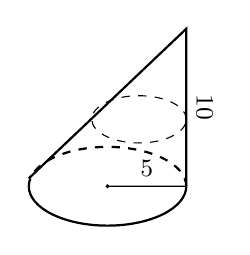
\begin{tikzpicture}[scale=.5]
\begin{scope}[xscale=2]
%\draw [thick](0,0) circle (1);
\draw [thick] (-1,0) arc (180:360:1);
\draw [thick,dashed] (1,0) arc (0:180:1);
\draw [dashed] (.4,1.7) circle (.6);
\end{scope}

\draw [fill=black] (0,0) circle (1pt) -- node [pos=.5,above] {\small 5} (2,0);
%\draw (0,0) -- node [pos=.5,rotate=90,above] {\small 10} (0,4);
\draw [thick] (-2,0.2) -- (2,4)-- node [pos=.5,rotate=-90,above] {\small 10}(2,0);
\end{tikzpicture}
}
{The cross--sections of this cone are the same as the cone in Exercise \ref{ex_07_02_ex_18}. Thus they have the same volume of $250\pi/3$ units$^3$.
}
